\documentclass[11pt]{article}
\usepackage{geometry}                % See geometry.pdf to learn the layout options. There are lots.
\geometry{letterpaper}                   % ... or a4paper or a5paper or ... 
%\geometry{landscape}                % Activate for for rotated page geometry
%\usepackage[parfill]{parskip}    % Activate to begin paragraphs with an empty line rather than an indent
\usepackage{graphicx}
\usepackage{amsmath}
\usepackage{amssymb}
\usepackage{epstopdf}
\usepackage{hyperref}
\DeclareGraphicsRule{.tif}{png}{.png}{`convert #1 `dirname #1`/`basename #1 .tif`.png}

\newtheorem{claim}{Claim}

\title{Modular iPOMDPs for HRL}
\author{Momchil}
%\date{Nov 2, 2017}                                           % Activate to display a given date or no date

\begin{document}
\maketitle
%\section{}
%\subsection{}






\section{Background} 


\subsection{Reinforcement Learning and Markov Decision Processes}

In reinforcement learning (RL), tasks are traditionally represented as Markov decision processes (MDPs) \cite{Sutton1998} and we will use those two terms interchangably. We define an MDP as a tuple $(\mathcal{S}, \mathcal{A}, T, R, I, \mathcal{F})$ where:
\begin{itemize}
\item $\mathcal{S}$ is a set of states that the agent can occupy,
\item $\mathcal{A}$ is a set of actions that the agent can perform in those states,
\item $T(\cdot|s,a)$ is a distribution of next states, such that $T(s'|s,a)$ is the probability that the agent ends up in state $s' \in \mathcal{S}$ after executing action $a \in \mathcal{A}$ in state $s \in \mathcal{S}$,
\item $R(s,a)$ is the amount of reward an agent obtains after executing action $a$ in state $s$,
\item $I(\cdot)$ is a distribution of initial states in which the agent may start the task,
\item $\mathcal{F}$ is a set of terminal states in which the task is completed.
\end{itemize}

The agent begins the task in state $s_0 \sim I$. At each time step $t$, the agent performs action $a_t$ that takes it from state $s_t$ to state $s_{t+1} \sim T(\cdot|s_t,a_t)$ and receives reward $r_t \sim R(s_t, a_t)$. The agent is said to follow a policy $\pi$ if it chooses its actions according to $a_t \sim \pi(\cdot|s_t)$.

For a fixed policy $\pi$, the state-value function $V_\pi(s)$ represents the total expected discounted reward for each state $s$. It is the sum of all future rewards that the agent will receive, on average, if it starts in state $s$ and follows $\pi$:

\[
V_{\pi}(s) = \mathbb{E}_{\pi} \left[  \sum_{t=0}^{\infty} \gamma^{t} r_t \middle| s_0 = s \right] ,
\]

where $\gamma$ is the discount rate which determines the present value of future rewards. The goal of the agent is to select an optimal policy $\pi^*$ that maximizes $V_{\pi^*}(s)$. The optimal value function $V_{\pi^*}(s)$ satisfies the Bellman optimality equation \cite{Bellman1957}:

\begin{align*}
V_{\pi^*}(s) = \max_a  \left\{ R(s,a) + \gamma \sum_{s'} V_{\pi^*}(s') \,\, T(s'|s,a) \right\} 
\end{align*}

The Bellman equation serves as a basis of a number of algorithms for solving optimal control problems.

\subsubsection{RL in the Brain}

RL algorithms often fall into one of two broad categories: model-free algorithms, in which the agent learns $V_\pi$ directly; and model-based algorithms, in which the agent learns $R$ and $T$ to compute $V_\pi$.  Computational cognitive neuroscience has borrowed this dichotomy as a formal description of the distinction between habitual and goal-directed behaviors \cite{Dolan2013}. Model-free accounts of habitual behaviors posit that animals learn automatic responses to stimuli if they tend to lead to rewarding outcomes. Model-based accounts of goal-directed behaviors posit that animals learn the statistics of the environment independently of the rewards.

Model-free accounts are less computationally intensive, however they require many training examples and have to be re-trained whenever the reward distribution changes. This is consistent with empirical observations that overtrained animals exhibit fast reaction times and rigid behavioral patterns that tend to persist even reward contingencies change. Model-free accounts are further bolstered by the hallmark discovery that the phasic firing of midbrain dopaminergic neurons closely tracks the model-free reward prediction error (RPE) signal.

Model-based accounts, on the other hand, predict that agents will flexibly adapt to changes in reward distributions, at the cost of slower reaction times due to the greater computational complexity. Model-based accounts explain phenomena such as latent learning and accord with the intuition that people don't have to learn a new policy, say, every time they go shopping for different groceries.

\subsection{Hierarchical Reinforcement Learning and Semi-Markov Decision Processes}

A long-standing challenge for traditional RL is the combinatorial explosion that occurs when planning and learning take place over long time horizons. This challenge been addressed by hierarchical reinforcement learning (HRL), which breaks down the problem into sub-problems at multiple levels of abstraction.

One strand of HRL extends the agent's action repertoire to include \textit{options} \cite{Sutton1999} -- temporally-extended sequences of actions, sometimes referred to as subroutines, partial policies, or macro-actions. Each option consists of a sequence of actions that are executed as a single behavioral unit. Actions in the original MDP are referred to as \textit{primitive actions}, in order to distinguish them from options.

Formally, including options turns the underlying MDP into a discrete-time semi-Markov decision process (SMDP), which allows transitions between states to take variable amounts of time. Thus we augment the original MDP with the following definitions:

\begin{itemize}
\item $\mathcal{O}$ is a set of options,
\item $\pi_o$ is a policy for each option $o \in \mathcal{O}$, such that while $o$ is being executed, actions are selected according to $a \sim \pi_o(\cdot|s)$,
\item $\mathcal{F}_o$ is a set of subgoal states for each option $o$, such that $\pi_o$ terminates when reaching any one of those states,
\item $T(\cdot,\cdot|s,o)$ is a joint distribution of terminal states and step counts for each option $o$, such that $T(s',t|s,o)$ is the probability that the agent ends up in subgoal state $s' \in \mathcal{F}_o$ exactly $t$ time steps after executing option $o \in \mathcal{O}$ in state $s \in \mathcal{S}$,
\item $R(s,o)$ is the total expected discounted reward for starting in state $s$ and executing option $o$.
\end{itemize}

The rewards can be computed as:

\begin{align*}
R(s,o) = \mathbb{E} \left[ \sum_{t=0}^\infty \gamma^t r_t \middle| s_0 = s, a_t \sim \pi_o \right]
\end{align*}

It is also convenient to define a discounted distribution of subgoal states \cite{Sutton1999}:

\begin{align*}
T_\gamma(s'|s,o) = \sum_{t=0}^\infty T(s',t|s,a) \gamma^t
\end{align*}

In the SMDP, the agent follows a policy $\mu$ defined over options, such that options are chosen according to $o_t \sim \mu(\cdot|s_t)$. The Bellman equation for the optimal options policy $\mu^*$ thus becomes:

\begin{align*}
V_{\mu^*}(s) = \max_o  \left\{ R(s,o) + \sum_{s'} V_{\mu^*}(s') \,\, T_\gamma(s'|s,o) \right\} 
\end{align*}

An options policy $\mu$ in the SMDP uniquely determines a \textit{flat policy} $\pi$ consisting solely of primitive actions in the original MDP. Thus any solution of the SMDP can be mapped back to a solution in the original MDP.

Introducing options allows agent to perform ``jumps'' in the state space. When considering an option $o$, the agent only needs to compute the value of its subgoal states $s' \in \mathcal{F}_o$, without computing the values of intermediate states that will be traversed while executing the option. If the subgoals and the options policies are chosen appropriately, exploration and planning can be performed much more efficiently by allowing the agent reason over short sequences of options, rather than over long sequences of primitive actions.

\subsubsection{HRL in the Brain}

In addition to its computational benefits, HRL provides an appealing account of habitual behaviors \cite{Botvinick2008} that competes with model-free RL. Model-free RL fails to capture habits which unfold as sequences of actions in response to a single cue, disregarding intervening cues \cite{Dezfouli2013}. It also fails to specify how habitual responses can be generalized across multiple task contexts.

Options as defined in HRL map nicely to habitual action sequences and their neural substrates. Research on rodents has implicated striatal and midbrain neurons in the formation and initiation of habitual action sequences, with task-bracketing activity emerging over the course of training in both regions \cite{Smith2013, Jin2014}. In these tasks, ``bumps'' of neural activity emerge at key decision points during the trial (e.g., at the trial start or at maze junctions), while activity is generally low in the remainder of the trial (e.g., while running straight). Similar task-bracketing activity has also been observed in birds and primates, suggesting a conserved neural implementation \cite{Smith2013}. The acquisition, initiation and termination of options in HRL may account for these diverse findings.

Additionally, the HRL framework has been directly supported by both behavioral \cite{Botvinick2014} and neural evidence \cite{Ribas-Fernandes2011}. It is also consistent with our intuition that people can plan over different time scales (e.g., go shopping, pick up the kids, etc.) without being bogged down by the details (e.g., get up, turn left, step forward, etc.).


\subsection{Option Discovery and Transfer}

The traditional HRL does not specify how options are transferred across tasks. Intuitively, under some circumstances, transferring an option from a previous task would speed up learning on a novel task (for example, learning to make a cup of coffee after learning to make a cup of tea). In other instances, learning a new task might be inhibited by previously acquired options, such as the tendency to get stuck in pre-existing ways of thinking that preclude creative solutions to new problems, a phenomenon known as the Einstellung effect \cite{Bilalic2008}. HRL does not make it clear why an agent faced with a new task would choose to execute an option acquired in a previous task, particularly if the state space of the new task is different. The problem of transferring behaviors from a source task to a target task has been investigated in the field of transfer learning and is often solved via an explicit inter-task mapping between states in the two tasks \cite{Taylor2009}. This mapping is often supplied manually or is discovered offline via batch heuristic methods which lack biological plausibility.

Furthermore, HRL fails to specify how options are learned in the first place, with most HRL accounts assuming a pre-specified set of options \cite{Botvinick2008}. The problem of discovering useful options has traditionally been addressed in an ad-hoc fashion, often by breaking down a task into multiple sub-tasks and defining the optimal solution to each sub-task as a separate option. The sub-tasks are often defined either by manually designating certain states as subgoal states using internal rewards (``pseudo-rewards''), or by partitioning the original task space based on the topology of the state transition structure (for example, by identifying ``bottleneck'' states such as doorways, or clusters of interconnected states such as rooms) \cite{Botvinick2008}. Solway et al. \cite{Solway2014} proposed a more principled solution based on Bayesian model selection. In their study, they showed that useful options can be learned by considering an ensemble of tasks occurring in the same environment. Human behavior was consistent with a decomposition of the environment into sub-tasks, each solved by a corresponding option, such that the resulting task hierarchy yields the most parsimonious explanation of optimal behaviors in the full task ensemble.

Even though it is limited by strong assumptions about the state space and the transition dynamics, the approach of Solway et al. highlights the importance of explicitly considering a distribution of tasks. In fact, most heuristic approaches to option discovery implicitly assume a task distribution, often by assuming that each accessible state has equal probability of being the start state or the goal state. To illustrate why option discovery only makes sense in the context of ensembles of tasks, consider what would happen if the agent only ever faced a single task in the world: it could then just learn the optimal policy for that one task using regular RL. Options in the HRL sense would thus be unnecessary as the entire policy would be executed automatically, like a single option. Options thus imply a world with multiple tasks. However, if those tasks were completely unrelated, options would again not make sense as the agent would have to learn a separate policy for each task from scratch, much like in the single-task scenario. In order for the agent to be able to learn useful options that can be transferred across tasks, there must be a shared structure between those tasks. While this point may seem trivial, we believe it lies at the crux of understanding how people and animals acquire their rich repertoire of habitual behaviors.

In order to understand how options are learned and facilitate performance on novel tasks, it is therefore necessary to define a probability distribution over tasks in the environment. Crucially, this distribution of tasks would be highly structured \cite{Botvinick2015}, such that tasks are grouped into families of tasks that share certain parameters which are not directly observable. Option discovery would thus correspond to a particular kind of hidden state inference, where the hidden state refers to the parameters that govern the distribution of tasks.

\subsection{Multi-task Reinforcement Learning}

\begin{figure}
\centering
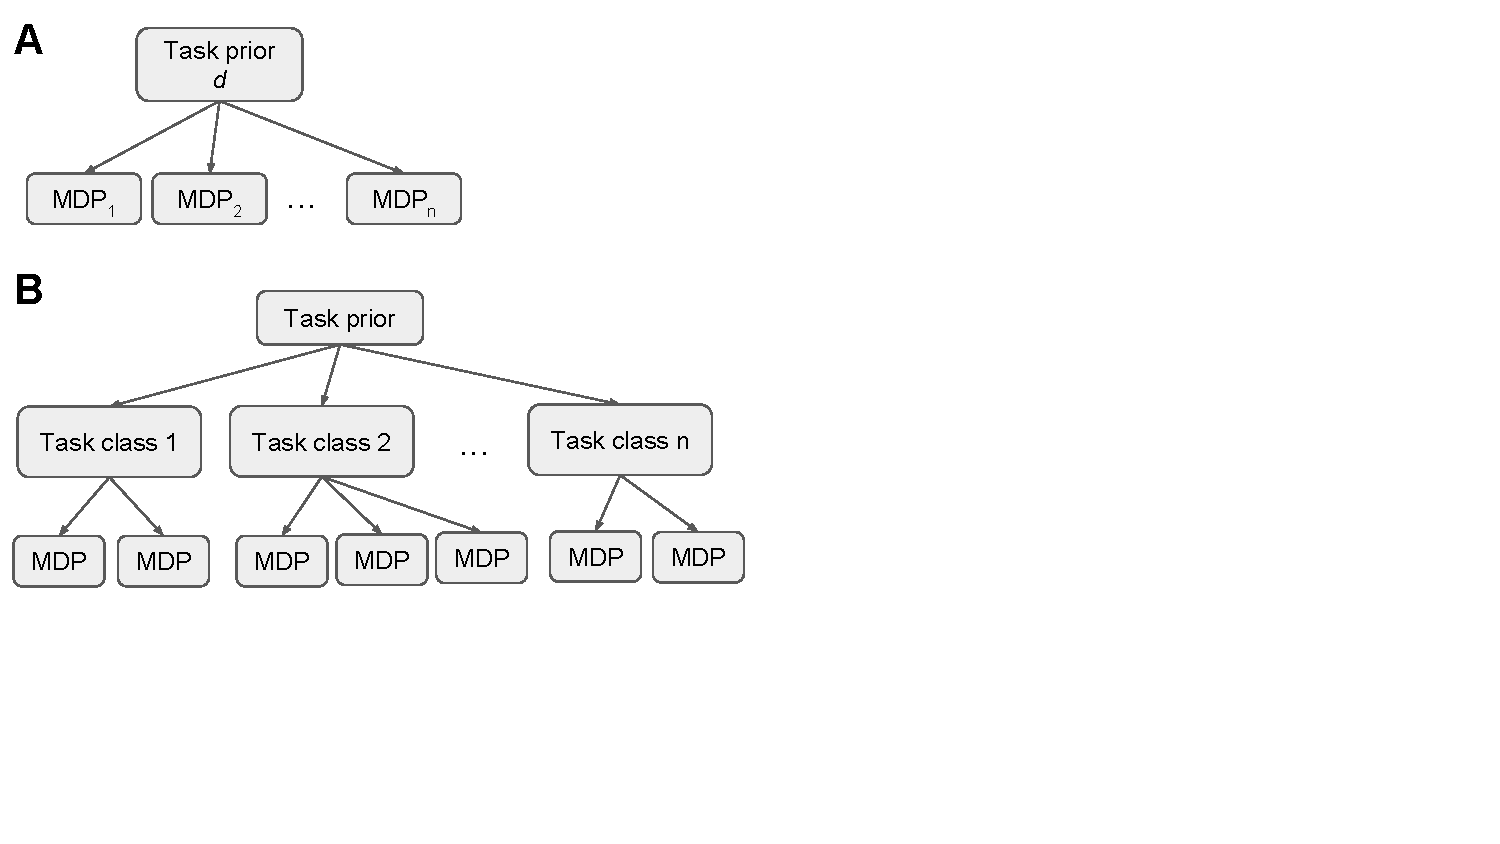
\includegraphics[scale=0.7,  trim = 0 120 400 10]{figures/wilson.pdf}
\caption{(A) The MTRL framework, (B) MTRL with classes of tasks. Adapted from \cite{Wilson2007}.}
\label{fig:mtrl}
\end{figure}

The problem of optimizing behaviors for a set of tasks (MDPs) drawn from a common distribution is the focus of multi-task reinforcement learning (MTRL) (Figure~\ref{fig:mtrl}A). In MTRL, MDPs are assumed to be drawn from the same prior distribution. Experiencing a sequence of MDPs can allow the agent to infer the hidden parameters of the distribution and to quickly discover the optimal policy for a new MDP drawn from the same distribution. In its simplest instantiation, MTRL allows the agent to learn a ``library'' of MDPs and reuse policies from MDPs it has seen in the past.

Wilson et al. \cite{Wilson2007} extended this framework to include \textit{classes} of tasks, where each class defines its own distribution of MDPs (Figure~\ref{fig:mtrl}B). Their model allows the agent to rapidly discover the structure of tasks similar to previous tasks, while simultaneously supporting the discovery of entirely new classes of tasks. Policies acquired in old tasks can thus be adapted to new tasks from the same class, while avoiding incorrect generalization to tasks from different classes.

\subsubsection{MTRL for HRL}

Wilson et al. showed how MTRL can be used when tasks share the same transition structure $T$, while other features such as the goal location and reward distributions vary. While this begins to address the question of policy transfer across MDPs, it leaves open several questions:

\begin{itemize}
\item How does ambiguity between MDPs arise? Traditional tabular MDPs assume that the agent is fully aware of what state it is in, which implies it is also fully aware of which MDP it is in. In order to be able to perform inference over MDPs, it must be the case that states are in some sense ``shared'' across MDPs, or at least ``look similar''.
\item What are the distributions over MDPs? Intuitively, they should be generic enough to capture a wide variety of tasks that agents may encounter in the world, while being constrained enough to facilitate efficient learning and generalization.
\item Why would options arise? In order to be able to define useful options and convert a given MDP into an SMDP, there must be some form of modular or subtask structure build into the MDP.
\item Why would options be transferred? In order to transfer options, the modules or subtasks need to be shared across MDPs.
\end{itemize}

We address the first question by appealing to the formalism of partially observable Markov decision processes (POMDPs), in which states are not directly observable but instead define distributions over observations. The agent must thus infer which state it is in based on these observations. In MTRL with POMDPs \cite{Li2009}, the agent additionally infers which POMDP it is in.

We address the second question using infinite POMDPs (iPOMDPs) \cite{DoshiVelez2009}, which allow the agent to flexibly adapt to environments with different state spaces.

We address the third question by constraining the iPOMDPs to a particular modular structure, such that states are grouped into \textit{modules}, sometimes referred to as communities or blocks or states. This is a novel contribution of our work.

We address the last question by allowing the structure and properties of these modules to be shared across different iPOMDPs.


\subsection{Partially Observable Markov Decision Processes}

\begin{figure}
\centering
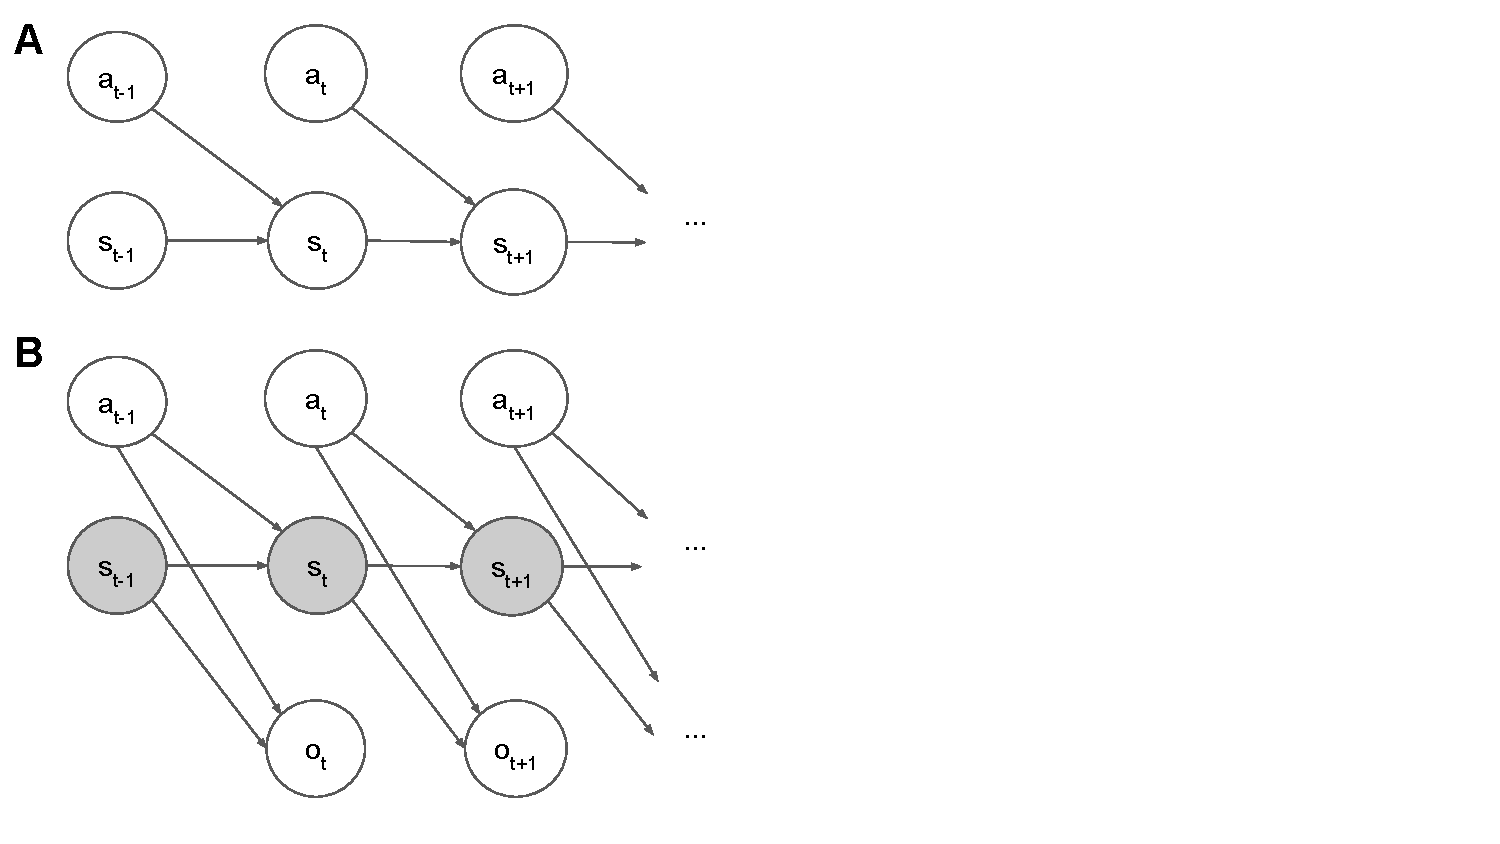
\includegraphics[scale=0.7,  trim = 0 10 400 10]{figures/pomdp.pdf}
\caption{(A) A time slice of an MDP showing the dependence between successive states and actions. (B) A time slice through the POMDP. Grey circles indicate that states are not directly observable.}
\label{fig:pomdp}
\end{figure}

Partially observable Markov decision processes (POMDPs) are useful for modeling environments in which states are not directly observable but rather generate observations, which the agent must use to infer the underlying hidden states (Figure~\ref{fig:pomdp}B). POMDPs extend MDPs by including the following:

\begin{itemize}
\item $\Omega$ is a set of observations,
\item $O(\cdot|s,a)$ is a distribution of observations, such that $O(o|s,a)$ is the probability of seeing observation $o \in \Omega$ after executing action $a \in \mathcal{A}$ in state $s \in \mathcal{S}$.
\end{itemize}

In POMDPs, the agent gets an observation after each action, so the agent's history is now a sequence of the form $\mathbf{h}_t = [o_0, a_0, o_1, a_1, o_2, a_2 ... a_{t-1}, o_t]$. The agent's history induces a probability distribution over the current state it is in:

\begin{align*}
b_t(s_t) = P(s_t | o_0, a_0 ... a_{t-1}, o_t)
\end{align*}

This summary statistic is known as a \textit{belief state}. It obeys the Markov property and can be updated recursively at each time step using Bayes' rule:

\begin{align*}
b_{t+1}(s_{t+1}) &=& P(s_{t+1} | o_0, a_0 ... a_t, o_{t+1})  \\
&=& \sum_{s_t}  T(s_{t+1} | s_t, a_{t+1}) \,\, P(s_t | o_0, a_0 ... a_t, o_{t+1}) \\
&\propto&  \sum_{s_t}  T(s_{t+1} | s_t, a_{t+1})  \,\, P(o_{t+1} | o_0, a_0 ... a_t, s_t) \,\, P(s_t | o_0, a_0 ... a_{t-1}, o_t) \\
&=& \sum_{s_t}  T(s_{t+1} | s_t, a_{t+1}) \,\, O(o_{t+1} | s_t, a_t) \,\, b_t(s_t) \\
\end{align*}

Rewards are treated as additional observations (omitted here to keep the notation uncluttered).

Now we can define MTRL using POMDPs \cite{Li2009}. Different POMDPs generate similar observations, creating ambiguity between POMDPs and necessitating inference over multiple POMDPs.

\subsubsection{POMDPs in the Brain}

Recent work \cite{Starkweather2017} using a task in which stimuli provide ambiguous information about the true state of the environment showed that the activity of midbrain dopaminergic neurons corresponds to the RPE computed on the inferred hidden state of the environment, consistent with a POMDP representation of the task.

\subsection{Infinite POMDPs}

In order to allow agents to learn a diverse set of tasks with different state spaces and transition functions, we turn to the formalism of infinite POMDPs (iPOMDPs) \cite{DoshiVelez2009}. This extends POMDPs in two ways. First, the transition probabilities $T$ are themselves treated as random variables with their own probability distributions. The unknown transitions $T$ together with the hidden state $s$ thus form an expanded hidden \textit{hyperstate} \cite{Duff2002}. This allows the agent to learn a POMDP with any arbitrary transition structure. Second, a nonparametric prior is defined over $T$, which allows for an unbounded number of states and transitions between them.

Formally, we generate a model from the iPOMDP prior in the following steps: 

\begin{itemize}
\item A state ``popularity'' vector $\bar{T}$ is drawn from a stick-breaking process (GEM) \cite{Teh2006} with concentration parameter $\alpha_0$, such that $\bar{T}(s')$ corresponds to the average probability that a transition will lead to state $s'$. It can be thought of as the average transition distribution.
\item A transition probability vector $T(\cdot | s,a)$ is drawn from a Dirichlet process (DP) \cite{Teh2006} with concentration parameter $\alpha_1$ and base distribution $\bar{T}$ for each state-action pair $(s,a)$.
\item An observation distribution $O(\cdot|s,a)$ is drawn from a base distribution $H_O$ for each state-action pair $(s,a)$.
\item A reward distribution $R(\cdot|s,a)$ is drawn from a base distribution $H_R$ for each state-action pair $(s,a)$.
\item States $s_t$, observations $o_t$, and rewards $r_t$ are drawn as usual from their corresponding distributions.
\end{itemize}

The steps can be summarized as:

\begin{align*}
\bar{T} \sim \text{GEM}(\alpha_0)  		&& \text{average transition distribution} \\
T(\cdot | s,a) \sim \text{DP}(\alpha_1, \bar{T})		 && \text{transition distributions}\\
O(\cdot | s,a) \sim H_O 				&& \text{observation distributions}\\
R(\cdot | s,a) \sim H_R 				&& \text{reward distributions}\\
s_t \sim T(\cdot | s_{t-1},a_{t-1}) 		&& \text{states}\\
o_t \sim O(\cdot | s_{t-1}, a_{t-1})		&& \text{observations} \\
r_t \sim R(\cdot | s_{t-1}, a_{t-1})		&& \text{rewards} 
\end{align*}

The popularity vector $\bar{T}$ and the transition vectors $T(\cdot | s,a)$ are of infinite size. However, the generative process favors a small number of states, and hence most of the probability mass will be concentrated on low-numbered states. The extent to which the model prefers ``small'' states is controlled by the concentration parameter $\alpha_0$. The concentration parameter $\alpha_1$ determines the similarity between each transition distribution $T(\cdot | s,a)$ and the mean distribution $\bar{T}$. 

Importantly, since the agent can only perceive a finite number of observations during its lifetime, it will only ever need to learn about a finite number of states.

An example iPOMDP is shown in Figure~\ref{fig:nested}A.




\subsection{Motivating Examples}

\begin{figure}
\centering
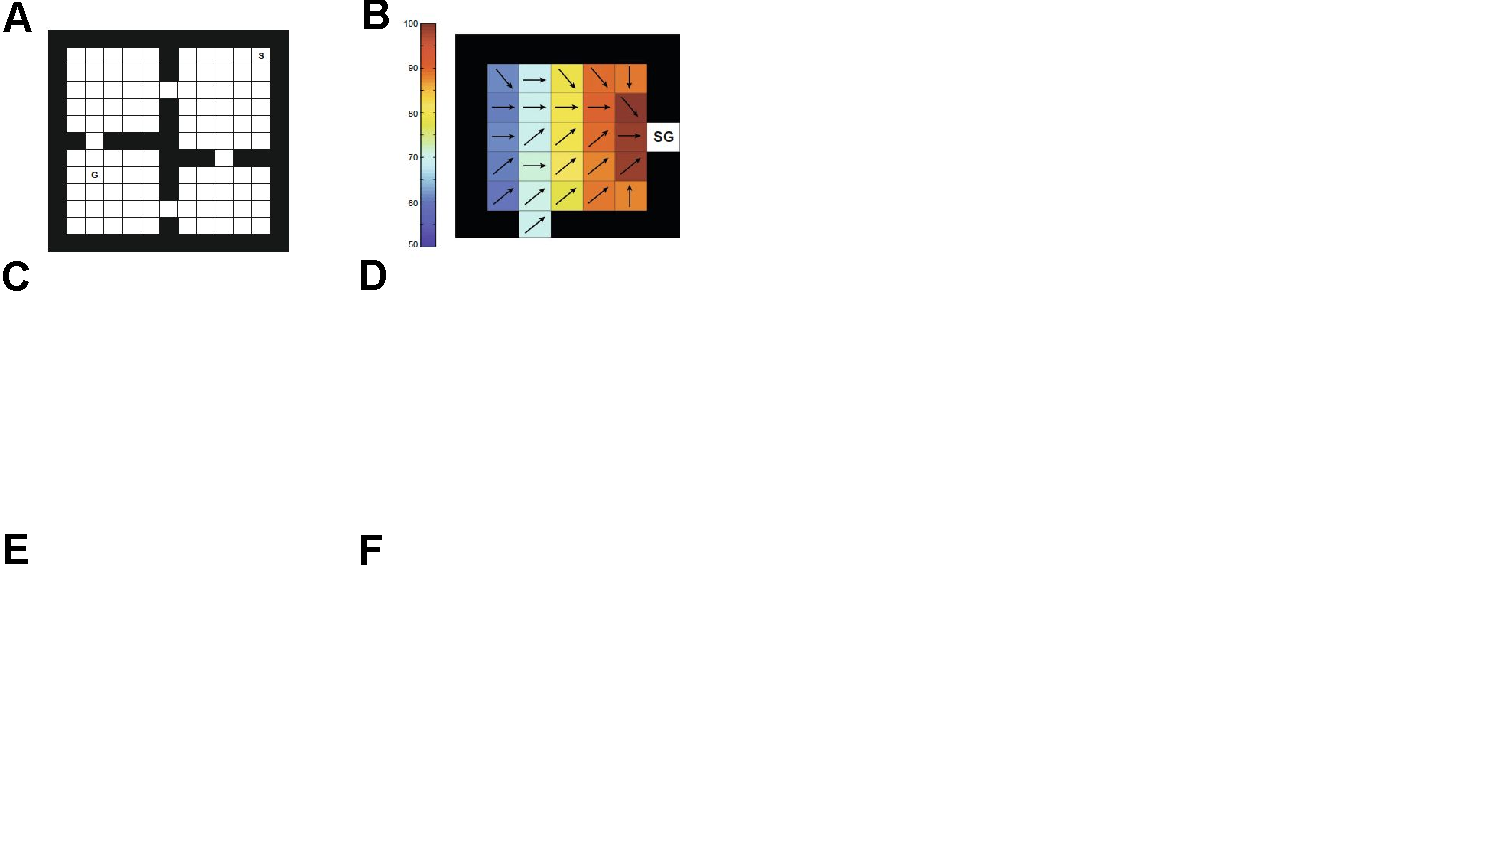
\includegraphics[scale=1,  trim = 20 20 10 10]{figures/examples.pdf}
\caption{(A) Rooms domain from \cite{Sutton1999}, adapted from \cite{Botvinick2008}. G, goal state, S, starting state. (B) Upper left room with its corresponding option policy (arrows) leading to the subgoal state (SG). Colors indicate option-specific state values. (C) Transition structure in a rooms domain, with transitions averaged over all four primitive actions (i.e. assuming a random walk). (D) Taxi domain from \cite{Dietterich2000}. (E) Transition structure in a taxi domain for given pickup and drop-off location (averaged over all actions). (F) Graph studied by Schapiro et al. \cite{Schapiro2013}. (G) Corresponding transition structure. (H) Graphs from Solway et al. \cite{Solway2014}. (I) Corresponding transition structures.}
\label{fig:examples}
\end{figure}

While the ultimate goal of this project is to design a generative model and inference machinery for a wide range of natural tasks, it is helpful to consider a few illustrative examples of constrained tasks used to study HRL and actions sequences.

\subsubsection{Machine Learning}

\paragraph{Rooms domain} A popular task used to illustrate HRL is the rooms domain (Figure~\ref{fig:examples}A, B, and C), which consists of a grid world in which some locations (states) are passable while others are not, dividing the space into rooms. There are four primitive actions: up, down, left, right. Transitions are deterministic and there is often a single goal state in which the task terminates. Usually any transition to the goal state gives some fixed reward, while all other transitions yield zero reward. Alternatively, all states have a negative reward associated with them, with the exception of the goal state which has zero reward. In both cases, the optimal policy is the shortest path from the agent's starting state to the goal state.

In such tasks, options arise naturally, with subgoals corresponding to the doorways between the rooms. If the reward is not in the same room as the agent, then it would have to go explore an adjacent room as fast as possible. Thus it helps to have option policies that lead to the exit of each room from any location within that room. That way the agent can directly perform the option ``go to doorway X'' and just follow the corresponding option policy.

\paragraph{Taxi domain}

Another classic task used to study HRI is taxi domain \cite{Dietterich2000} (Figure~\ref{fig:examples}D and E). It is a 5-by-5 grid world in which there are four passenger pick up / drop off locations. Time is broken into episodes. In each episode, there is a passenger in one of the four locations (the pickup location) who desires to go to another one of the four locations (the drop-off location). The taxi (agent) starts in a random location and has to navigate to the pickup location, pick up the passenger, navigate to the drop-off location, and drop off the passenger. The rewards are set up to encourage the shortest path. There are six primitive actions: up, down, left, right, pick up, drop off. 

In this domain, it is useful to have an option for navigating to each of the four designated pickup / drop-off locations. Notice that the structure of the taxi domain resembles many real-world tasks in which an agent needs to perform some action in one location before performing another action in a different location, such as picking up a key to unlock a door.


\subsubsection{Humans}

\paragraph{Community structure}

Schapiro et al. \cite{Schapiro2013} performed a study in which participants experienced random walks in a graph and had to press a button whenever they perceived a ``boundary'' event (Figure~\ref{fig:examples}F). Participants pressed more on transitions between clusters (or ``communities'') of interconnected nodes in the graph, suggesting that they intuited the underlying structure. The study further showed that this community structure is reflected in neural activity, with some brain areas showing similar activity for states in the same community.

Even though there are no actions in this task, one can imagine that if it were converted to a navigation task with a randomly chosen start state and goal state, it would be useful to have options for navigating between the communities. Solway et al. \cite{Solway2014} showed that, under these assumptions, this is indeed the optimal subtask decomposition of this domain.

Solway et al. \cite{Solway2014} performed a study in which participants were asked to navigate in different domains with community structure. In their first experiment (Figure~\ref{fig:examples}H, top), participants learned the adjacency relations among locations in a virtual town. When asked to pick an optimal location for a bus stop in order to speed up deliveries between locations, participants tended to pick the locations corresponding to topological bottlenecks, suggesting that they discovered the community structure. In the second experiment, participants were explicitly asked to navigate between locations in a different domain (Figure~\ref{fig:examples}H, bottom). Participants were able to quickly indicate that the bottleneck states would lie on a shortest path between two random states, again indicating that they discovered the community structure.


\subsubsection{Rodents}

\begin{figure}
\centering
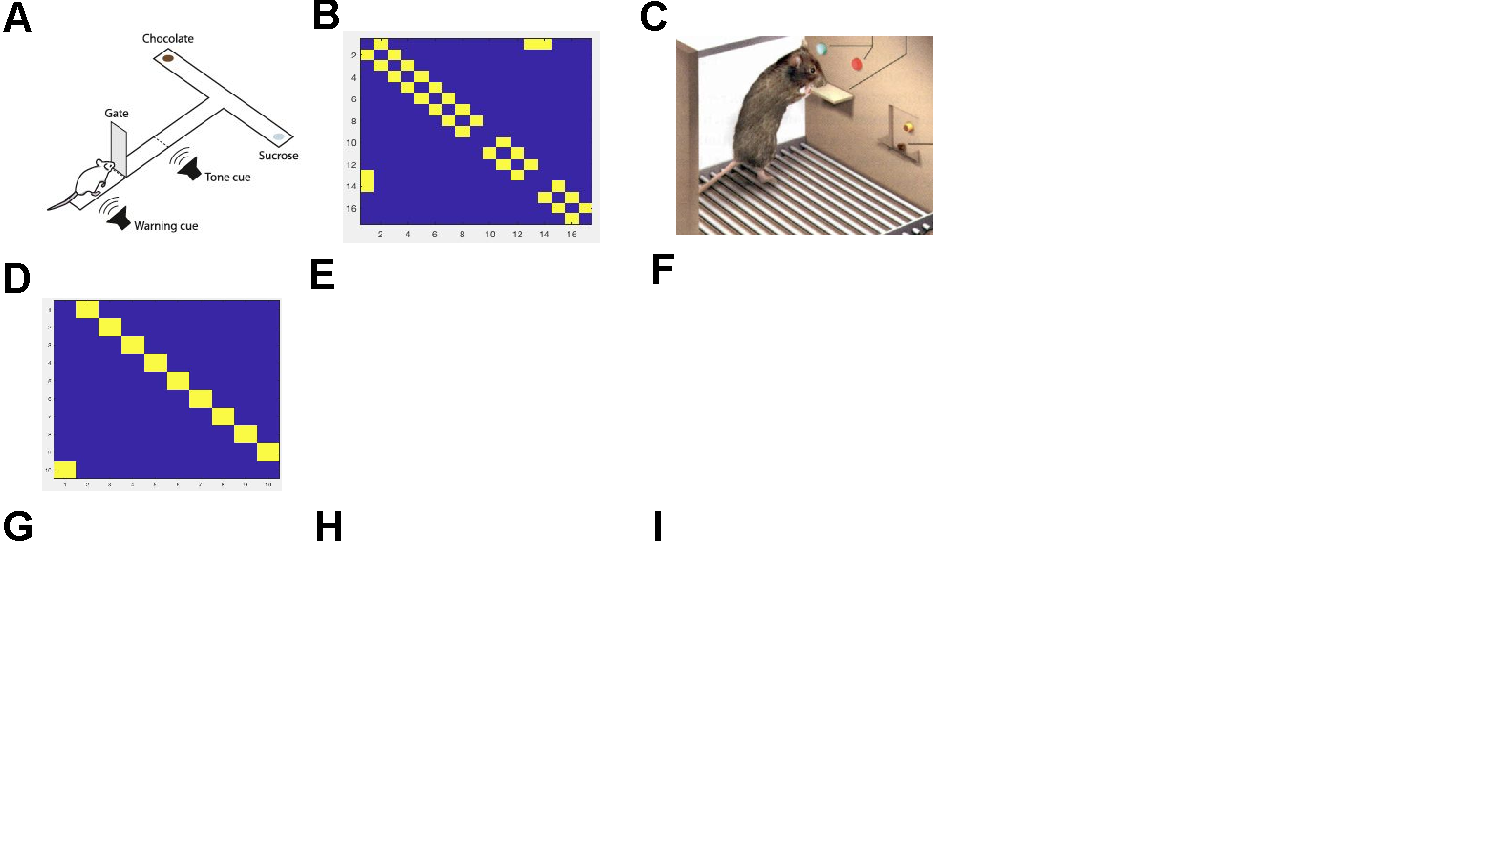
\includegraphics[scale=1,  trim = 20 20 10 10]{figures/examples2.pdf}
\caption{(A) T-maze from \cite{Smith2013b}. (B) Corresponding transition structure (averaged across actions) if the maze is broken down into discrete states akin to the rooms domain. (C) Lever pressing task from Jin et al. \cite{Jin2010}. (D) Corresponding transition structure, with state 1 = no sequence started, state 10 = at reward dispenser, and each lever press leading from state $n$ to state $n+1$. }
\label{fig:examples2}
\end{figure}

\paragraph{T-maze} 

The T-maze is frequently used to study habitual behavior in rodents \cite{Smith2013} (Figure~\ref{fig:examples2}A). Animals receive a cue and run down the long arm of the T-maze towards the junction. There is a reward in one of the end-arms, and the animal receives the reward if it turns to the correct arm.

The option in this simple task is defined by the subgoal state corresponding to the maze junction, which is the same both on left-turn and right-turn trials. Smith et al. \cite{Smith2013b} and others have shown that over the course of training, task-bracketing activity emerges in some brain regions of rats, with an increase in neural activity at the junction point of the maze in addition to the beginning and the end of the trial.

\paragraph{Lever pressing}

Jin et al. \cite{Jin2010} studied sequence formation using a lever-pressing task in which mice had to press a lever 8 times in sequence in order to receive a reward (Figure~\ref{fig:examples2}C).

In this self-paced task, a useful option policy would be pressing 8 times in a row. Jin et al. found neural signals corresponding to the initiation and termination of such sequences of lever presses.



\subsubsection{Monkeys}






\section{The Model}

\begin{figure}
\centering
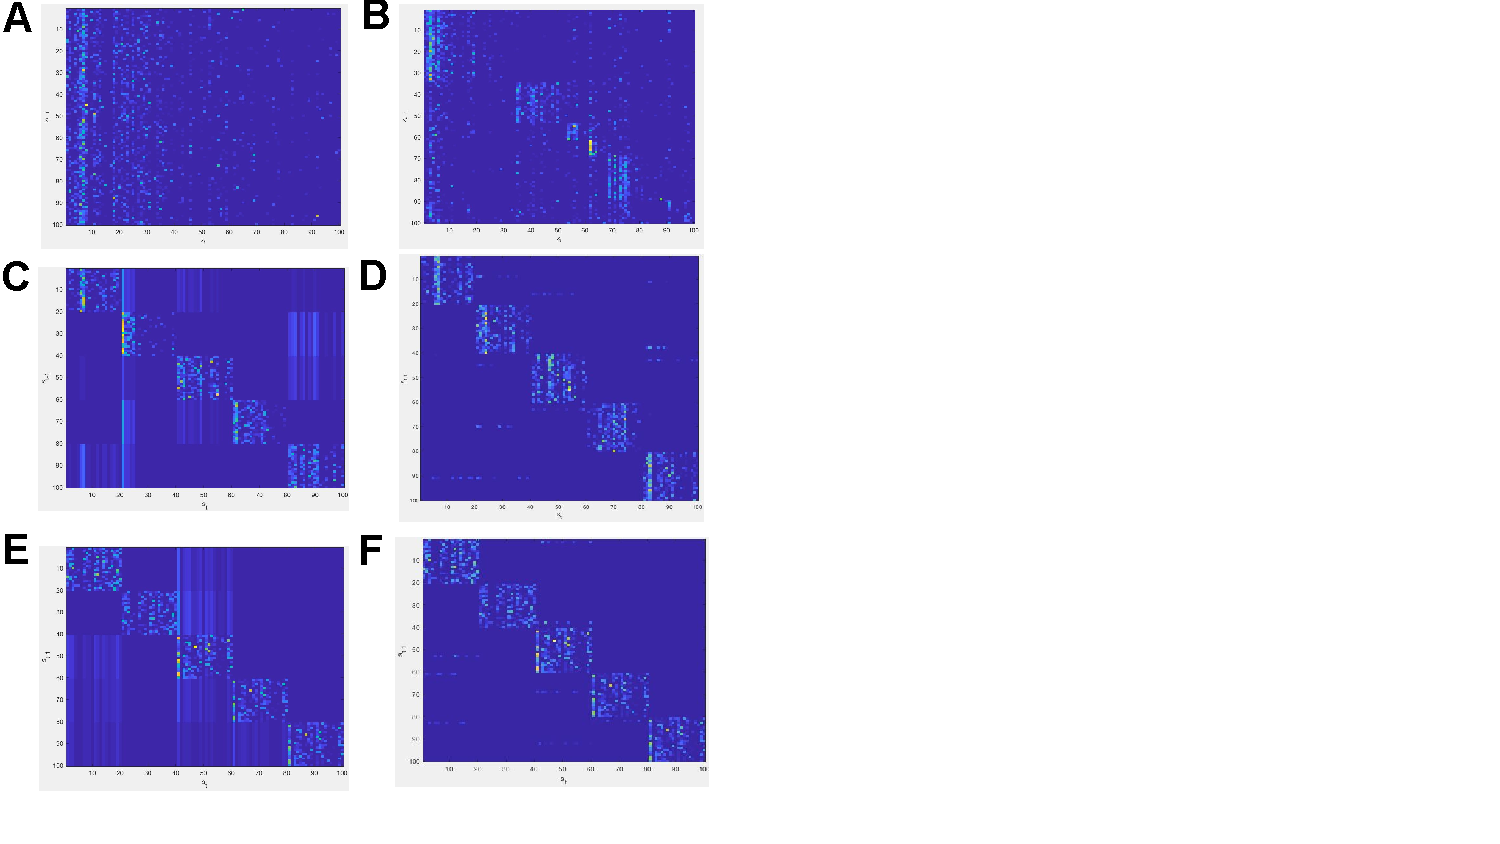
\includegraphics[scale=1,  trim = 0 20 400 10]{figures/nested.pdf}
\caption{(A) The transition probabilities $T(s_t| s_{t-1}, a_{t-1})$ for a fixed action $a_t$ in a iPOMDP sampled from the prior. (B) Modular iPOMDP with module-specific popularity vectors. (C) Two-layer iPOMDP. (D) Two-layer iPOMDP with subgoals. Notice the sparse off-diagonal transitions. (E) Two-layer iPOMDP with templates. Notice that the within-module transition structures of the first two modules (top left) are identical since they are taken from the same template. Similarly, the within-module transition structures of the last three modules (bottom right) are also identical but drawn from a different template. (F) Two-layer iPOMDP with subgoals and templates.}
\label{fig:nested}
\end{figure}

\subsection{Modular iPOMDPs}

Combining MTRL with iPOMDPs allows the agent to learn and transfer policies across tasks with arbitrary state spaces and transition structures. However, it is still unclear how options would arise in such a framework. Intuitively, options imply a certain modular structure, such that some parts of the state space have characteristic transition structures or observation distributions which are repeated across POMDPs or even within the same POMDP. Learning an appropriate sequence of actions in one of those modules will allow the agent to transfer it to other instances of the same module.




\subsubsection{Module-specific popularity vectors}

One way to incorporate modules in iPOMDPs is by extending block diagonal infinite hidden Markov models (BD-iHMMs) \cite{Stepleton2009}. Intuitively, each state is assigned to a module, and states from the same module tend to transition to states within the module more often than to states outside of the module. As an example, modules can be thought of as rooms, while states in each module can be thought of as locations within the room.

Formally, we can introduce the following:

\begin{itemize}
\item $\mathcal{M}$ is a set of modules,
\item $\bar{T}_m$ is a state popularity vector for each module $m \in \mathcal{M}$,
\item $z_s \in \mathcal{M}$ is the module that state $s \in \mathcal{S}$ belongs to.
\end{itemize}

To generate a modular iPOMDP:

\begin{itemize}
\item A module popularity vector $\beta$ is drawn from a stick-breaking process with concentration parameter $\gamma$.
\item A module assignment $z_s$ is drawn for each state $s$ from a categorial distribution defined by $\beta$.
\item An overall state popularity vector $\bar{T}$ is drawn from a stick-breaking process with concentration parameter $\alpha_0$.
\item A module-specific state popularity vector $\bar{T}_m$ is created for each module $m$. It is equal to $\bar{T}$, except with $\bar{T}_m(s)$ scaled by a factor of $(1 + \xi)$ for all states $s$ such that $z_s = m$. The whole vector $\bar{T}_m$ is then renormalized to sum to 1.
\item A transition probability vector $T(\cdot | s,a)$ is drawn from a DP with concentration parameter $\alpha_1$ and base distribution $\bar{T}_m$ for each state-action pair $(s,a)$, where $m = z_s$.
\item Reward distributions $R$, observation distributions $O$, states $s_t$, observations $o_t$, and rewards $r_t$ are drawn as for regular iPOMDPs.
\end{itemize}

The steps can be summarized as:

\begin{align*}
\beta \sim \text{GEM}(\gamma)   		&& \text{module popularities} \\
z_s \sim \beta   		&& \text{module assignments} \\
\bar{T} \sim \text{GEM}(\alpha_0)     		&& \text{average transition distribution} \\
C_m =  1 + \xi {\sum_s \bar{T}(s) \,\, \delta(z_s = m) }   		&& \text{normalization constant} \\
\bar{T}_m(s) = \begin{cases} \frac{1 + \xi}{C_m} \bar{T}(s)  \,\, \text{ if }  z_s = m \\  \frac{1}{C_m} \bar{T}(s) \,\, \text{ if } z_s \ne m \end{cases}     		&& \text{average transition distribution for each module} \\ 
T(\cdot | s,a) \sim \text{DP}(\alpha_1, \bar{T}_m), \text{ where } m = z_s 		 && \text{transition distributions}\\
O(\cdot | s,a) \sim H_O \\
R(\cdot | s,a) \sim H_R \\
s_t \sim T(\cdot | s_{t-1},a_{t-1}) \\
o_t \sim O(\cdot | s_{t-1}, a_{t-1}) \\
r_t \sim R(\cdot | s_{t-1}, a_{t-1}) 
\end{align*}

Unlike regular iPOMDPs, here there is a separate average transition distribution $\bar{T}_m$ for each module $m$. Importantly, that distribution is artificially skewed to prefer states within $m$. The parameter $\xi$ controls the bias for within-module transitions, with $\xi = 0$ leading to no bias. The concentration parameter $\gamma$ determines whether the prior is biased towards a small or a large number of modules.

An example modular iPOMDP is shown in Figure~\ref{fig:nested}B.

The module-specific average transition distributions would allow the model to discover the modular or ``community'' structure of tasks in the environment, something which is characteristic of human behavior \cite{Schapiro2013, Solway2014}. However, since each transition distribution $T(\cdot|s,a)$ is drawn independently (conditional on $\bar{T}_m$), each module will have its own unique transition structure. An option learned in one module would not apply to a different module.




\subsubsection{Two-layer iPOMDPs}

In order to facilitate the acquisition of options, modules need to be repeated, which is infeasible with the previous approach. The easiest way to achieve this is by treating modules as self-contained units. One way to accomplish this is by inducing a separate iPOMDP for each module, which would be ``nested'' in a higher-level iPOMDP defined over modules.

To illustrate this, consider the original iPOMDP formulation in which states induce distributions over observations. Now imagine that states are modules, and that the observations themselves are the states, with their own module-specific transition distributions.

Formally, we can generate a two-layer iPOMDP as follows:


\begin{itemize}
\item A \textbf{module} popularity vector $\bar{T}$ is drawn from a stick-breaking process with concentration parameter $\alpha_0$, such that $\bar{T}(m')$ corresponds to the average probability that a transition will lead to module $m'$.
\item A \textbf{module} transition probability vector $T(\cdot | m)$ is drawn from a DP with concentration parameter $\alpha_1$ and base distribution $\bar{T}$ for each module $m$, such that $T(m'|m)$ is the average probability that an action in a state in module $m$ will lead to a state in module $m'$.
\item A within-module \textbf{state} popularity vector $\bar{T}_{m}$ is drawn from a stick-breaking process with concentration parameter $\alpha_2$ for each module $m$, such that $\bar{T}_m(s')$ corresponds to the average probability that a transition within module $m$ will lead to state $s'$. This pertains to transitions to states within $m$ only.
\item A within-module \textbf{state} transition probability vector $T_m(\cdot|s,a)$ is drawn from a DP with concentration parameter $\alpha_3$ and base distribution $\bar{T}_{m}$ for each state-action pair $(s,a)$ within each module $m$. Thus $T_m(s'|s,a)$ is the probability of transitioning to state $s'$ after taking action $a$ in state $s$ within module $m$. Note that both $s$ and $s'$ belong to module $m$.
\item Global transitions $T(s'|s,a)$ across states (both within and across modules) are defined as follows. If both $s$ and $s'$ are in the same module $m$, then $T(s'|s,a)$ equals the within-module transition probability $T_m(s'|s,a)$, scaled by the probability that a module will transition to itself, $T(m|m)$. If $s$ and $s'$ belong to different modules $m$ and $m'$, respectively, then $T(s'|s,a)$ is taken to be the popularity of $s'$ in module $m'$, $\bar{T}_{m'}(s')$, scaled by the probability of a transition from $m$ to $m'$, $T(m'|m)$.
\item Reward distributions $R$, observation distributions $O$, states $s_t$, observations $o_t$, and rewards $r_t$ are drawn as for regular iPOMDPs.
\end{itemize}

The steps can be summarized as:

\begin{align*}
\bar{T} \sim \text{GEM}(\alpha_0)      		&& \text{module popularities}  \\
T(.|m) \sim \text{DP}(\alpha_1, \bar{T})      		&& \text{module transitions} \\
\bar{T}_{m} \sim \text{GEM}(\alpha_2)      		&& \text{within-module state popularities} \\
T_m(\cdot|s,a) \sim \text{DP}(\alpha_3, \bar{T}_m) ,\,\,\forall s \in m      		&& \text{within-module state transitions} \\
T(s'|s,a) = \begin{cases}  T_m(s'|s,a) \,\, T(m|m) & \text{ if } s, s' \in m \\  \bar{T}_{m'}(s') \,\, T(m'|m) & \text{ if } s \in m, s' \in m'  \end{cases}			&& \text{transitions between all states} \\
O(\cdot | s,a) \sim H_O \\
R(\cdot | s,a) \sim H_R \\
s_t \sim T(\cdot | s_{t-1},a_{t-1}) \\
o_t \sim O(\cdot | s_{t-1}, a_{t-1}) \\
r_t \sim R(\cdot | s_{t-1}, a_{t-1}) 
\end{align*}

As before, it makes sense to introduce a bias that favors transitions within modules by scaling $T(m|m)$ by a factor of $(1 + \xi)$:

\begin{align*}
T(m'|m) \leftarrow \begin{cases}  \frac{1 + \xi}{1 + \xi T(m|m)} \,\, T(m|m) \,\,\text{ if }m' = m    \\  \frac{1}{1 + \xi T(m|m)} \,\, T(m'|m)\,\,\text{ if }m' \ne m  \end{cases}
\end{align*}

Now each module has its own separate transition structure defined by $T_m$. Even though each module is still unique, this version of the model allows us to bias the prior towards repeated modules, which would naturally give rise to options.

An example of a two-layer iPOMDP is shown in Figure~\ref{fig:nested}C.





\subsubsection{Two-layer iPOMDPs with subgoals}

For options to arise, there need to be certain states which can be designated as subgoals. One common definition of subgoals is ``bottleneck'' states, such as doorways or passages, which in our framework would correspond to states which transition from one module to another. Intuitively, we want the cross-module transitions to be sparse (Figure~\ref{fig:examples}C,E,G,I, and Figure~\ref{fig:examples2}B,D), with a few states from one module (the subgoal or \textit{exit} states) transitioning to a few states to another module (the \textit{entrance} states). 

Two-layer iPOMDPs as defined above posit that each state from a given module $m$ has the same transition distribution for all states in another module $m'$, which is implausible (notice the off-diagonal structure in Figure~\ref{fig:nested}C).

We would like to define \textbf{cross-module} state transition distributions $T_{m,m'}(s'|s,a)$, specifying the probability of transitioning from state $s \in m$ to state $s' \in m'$ after taking action $a$ (for $m \ne m'$). We also want this distribution to be sparse, i.e. all probabilities would be zero for most states $s$, except for a few states $s$ (the exit states of $m$) which would transition to a few states $s'$ (the entrance states of $m'$). One way to achieve this is by selecting a single exit state $s_{m,m'}$ that acts as a ``bridge'' from module $m$ to module $m'$:

\begin{itemize}
\item An \textbf{exit state} probability vector $\bar{T}_{m,\cdot}$ is drawn from a GEM with concentration parameter $\alpha_4$, specifying which states in module $m$ are likely to be exit states.
\item An \textbf{entrance state} probability vector $\bar{T}_{\cdot,m'}$ is drawn from a GEM with concentration parameter $\alpha_5$, specifying which states in module $m'$ are likely to be entrance states.
\item A single \textbf{exit state} $s_{m,m'} \in m$ is chosen according to $\bar{T}_{m,\cdot}$ for each pair of distinct modules $m, m'$. Its transition distribution $T_{m,m'}(\cdot|s,a)$ to states $s' \in m'$ is then chosen according to a DP with base distribution $\bar{T}_{\cdot,m'}$ and concentration parameter $\alpha_6$.
\item Global transitions $T(s'|s,a)$ are modified accordingly.
\end{itemize}

Thus the overall two-layer iPOMDP generation process can be summarized as:

\begin{align*}
\bar{T} \sim \text{GEM}(\alpha_0)      		&& \text{module popularities}  \\
T(.|m) \sim \text{DP}(\alpha_1, \bar{T})      		&& \text{module transitions} \\
\bar{T}_{m} \sim \text{GEM}(\alpha_2)      		&& \text{within-module state popularities} \\
T_m(\cdot|s,a) \sim \text{DP}(\alpha_3, \bar{T}_m) ,\,\,\forall s \in m      		&& \text{within-module state transitions} \\
\bar{T}_{m,\cdot} \sim \text{GEM}(\alpha_4)      		&& \text{exit state popularities}  \\
\bar{T}_{\cdot,m'} \sim \text{GEM}(\alpha_5)      		&& \text{entrance state popularities}  \\
s_{m,m'} \sim \bar{T}_{m,\cdot}					&& \text{exit states}  \\
T_{m,m'}(\cdot|s,a) \sim \text{DP}(\alpha_6, \bar{T}_{\cdot,m'}),  \text{ for } s = s_{m,m'}      		&& \text{cross-module state transitions} \\
T(s'|s,a) = \begin{cases}  T_m(s'|s,a) \,\, T(m|m) & \text{ if } s, s' \in m \\  \bar{T}_{m,m'}(s'|s,a) \,\, T(m'|m) & \text{ if } s \in m, s' \in m'  \end{cases}			&& \text{transitions between all states} \\
O(\cdot | s,a) \sim H_O \\
R(\cdot | s,a) \sim H_R \\
s_t \sim T(\cdot | s_{t-1},a_{t-1}) \\
o_t \sim O(\cdot | s_{t-1}, a_{t-1}) \\
r_t \sim R(\cdot | s_{t-1}, a_{t-1}) 
\end{align*}

With the same additional bias for higher $T(m|m)$, favoring within-module transitions.

An example of a two-layer iPOMDP with subgoals is shown in Figure~\ref{fig:nested}D.

\paragraph{Transitions mixture}

While this definition of subgoals conforms nicely to the structure of some of the considered tasks, one exit state per module might be too restrictive. However, I'm not sure how to draw a set of exit states. The HDP formalism doesn't apply straightforwardly here as we need to draw a set of \textit{unique} states. Some variants:

\begin{itemize}
\item Treat exit states as ``observations'' and just keep drawing from the exit state distribution $\bar{T}_{m,\cdot}$. Would need an additional parameter to decide when to stop drawing (e.g. a Bernoulli distribution parameter). Also have to decide how to handle the repeats.
\item Decide for each state separately whether it's an exit state based on $\bar{T}_{m,\cdot}$ (e.g. a Bernoulli coin flip). Seems really wrong to use categorical probabilities as Bernoulli probabilities...
\item Make the cross-module transitions $T_{m,m'}(\cdot|s,a)$ into mixtures between what they are now and $\text{DP}(..., \bar{T}_{m'})$, i.e. what they would have been if $s$ and $s'$ were in the same module. So any state in $m$ can connect to any state in $m'$. But then we're losing the off-diagonal sparsity... Extra care must be taken to weigh down these transitions without weighing down the exit-entrance state transitions.
\end{itemize}


\subsubsection{Two-layer iPOMDPs with templates}

One way to bias the prior towards repeated structures to allow transition structures to be shared between different modules. Thus two different modules $m$ and $m'$ may have identical state transition structures $T_m \equiv T_{m'}$.

To accomplish this, it is convenient to introduce \textit{templates} $\tau$ that define unique transition structures $T_{\tau}$. Each module $m$ is assigned to a template $\tau$, resulting in $T_m \equiv T_\tau$. 

We introduce the following components to the two-layer iPOMDP generation process:

\begin{itemize}
\item $\bar{T}_\tau$ and $T_\tau$ are drawn in the same way as $\bar{T}_m$ and $T_m$, respectively, except defined for templates $\tau$ instead of modules $m$.
\item A template popularity vector $\beta$ is drawn from a stick-breaking process with concentration parameter $\gamma$.
\item A template assignment $z_m$ is drawn for each module $m$ from a categorial distribution defined by $\beta$.
\item $\bar{T}_m$ and $T_m$ are assigned equal to $\bar{T}_\tau$ and $T_\tau$, respectively, for the corresponding template $\tau = z_m$.
\end{itemize}

Hence instead of drawing $\bar{T}_m$ and $T_m$ for modules $m$, we now draw them for templates $\tau$ in the exact same manner:

\begin{align*}
\bar{T}_{\tau} \sim \text{GEM}(\alpha_2)  \\
T_\tau(\cdot|s,a) \sim \text{DP}(\alpha_3, \bar{T}_\tau) ,\,\,\forall s \in \tau
\end{align*}

Modules are assigned to templates according to:

\begin{align*}
\beta \sim \text{GEM}(\gamma) \\
z_m \sim \beta \\
\bar{T}_{m} \equiv \bar{T}_{\tau},  \text{ where } \tau = z_m \\
T_m(\cdot|s,a) \equiv T_\tau(\cdot | s,a), \text{ where } \tau = z_m 
\end{align*}

An example of a two-layer iPOMDP with templates is shown in Figure~\ref{fig:nested}E.

Templates would allow agents to quickly infer the transition structure in domains in which large portions of the state space are repeated. While this is unlikely in pure navigation tasks like the rooms domain, it is common in tasks with more complicated state spaces such as the taxi domain (Figure~\ref{fig:examples}E). Even in the rooms domain, most (Figure~\ref{fig:examples}C), a lot of the structure of the rooms is repetitive, and that could be ``templated'' out, with the remaining states assigned to ad-hoc modules. Templates would be useful in state spaces with community structure such as those considered by previous authors (Figure~\ref{fig:examples}G,I). They could also be useful in games with isomorphic structures in the state space, such as the Towers of Hanoi. Finally, repetitive structure also arises in rodent tasks, for example in tasks with two levers where a sequence of presses on each lever leads to a symmetric outcome (e.g. food pellet in the corresponding magazine).

\subsubsection{Two-layer iPOMDPs with templates and subgoals}

The iPOMDP with subgoals can easily be combined with templates. An example is shown in Figure~\ref{fig:nested}F.

\paragraph{Templated subgoals}

Additionally, module entrance and exit states could similarly be templated, with the probability vectors $\bar{T}_{m,\cdot}$ and $\bar{T}_{\cdot,m'}$ assigned to corresponding probability vectors $\bar{T}_{\tau,\cdot}$ and $\bar{T}_{\cdot,\tau'}$ (where $\tau = z_m$) that are drawn for templates instead of modules. In this way, modules of the same template will tend to have the same entrance and exit states (notice that we can only duplicate the distributions, since the actual entrance and exit states are drawn for pairs of modules).


\subsection{MTRL with two-layer iPOMDPs}

There are different ways to adapt two-layer iPOMDPs to the MTRL framework that will facilitate the acquisition and transfer of different kinds of options.

\subsubsection{Prior over tasks}

One convenient choice is a Chinese restaurant process (CRP) \cite{Teh2006} prior over tasks. Intuitively, we can think of time as being divided into discrete episodes (or trials). At the start of each episode, the agent is presented with a task, which is either identical to a task seen in a previous episode, or is an entirely new task. The CRP prior favors a rich-gets-richer dynamic whereby tasks which are selected frequently tend to be selected even more frequently.

Formally, if the distinct tasks are indexed by $k = 1..K$, then on episode $e$, the task is drawn according to: 

\begin{align*}
P(\text{task}_e = k | \text{task}_0, \text{task}_1 ... \text{task}_{e-1} ) \propto \begin{cases}  n_k  & \text{ if } k \le K \\ \alpha & \text{ if } k = K + 1\end{cases}
\end{align*}

where $K$ is the number distinct tasks presented so far, $n_k$ is the number of times task $k$ has been chosen before, and $\alpha$ is a concentration parameter.

In our case, the tasks are represented by two-layer iPOMDPs. During each episode, the agent can use the CRP prior to decide whether it is learning a new iPOMDP, or whether it is performing in a previously encountered iPOMDP.

\subsubsection{Shared templates}

In the framework presented so far, templates are defined separately for each iPOMDP. In order to allow the acquisition of options that apply across multiple iPOMDPs, we can allow templates to be shared across iPOMDPs. This can be done in a straightforward manner by drawing $\bar{T}_\tau$ and $T_\tau$ once and using them in all iPOMDPs. 

This would be useful for transferring options across tasks. If entrance/exit states are also included in the templates, then distributions over subgoals could also be shared. This would help in task which share parts of their transition structures. A few examples:

\paragraph{The taxi domain} Each module corresponds to the grid world for a given passenger (or no passenger) in the taxi (Figure~\ref{fig:examples}E). Since navigation is independent of the passenger, the grid transition structure is copied over exactly as is. Templates will be helpful for:

\begin{itemize}
\item within-task transfer (e.g. no need to learn how to navigate from scratch after picking up a passenger),
\item cross-task transfer if templates are shared across iPOMDPs (e.g. no need to learn how to navigate from scratch on episodes with different pickup / drop off locations),
\item cross-task transfer of subgoals, if the entrance and exit state distributions are part of the templates too. This will occur as the entrance/exit states will naturally map to pickup / drop off locations. After a few tasks, the agent will learn the four key locations as most likely entrance/exit points.
\end{itemize}

Crucially, templates will allow transfer if the state space is expanded further, such as adding extra pickup/drop off locations, or the need to refuel \cite{Dietterich1998}, or if the taxi is allowed to venture into neighboring grid worlds. The transition structure for navigating the grid world will just be copied over.

Shared templates will facilitate learning by shaping, i.e. by gradually introducing the agent to more complicated environments with tasks that gradually expand the state space of previously encountered tasks. By learning the appropriate templates in the initial tasks, the agent will be able to quickly learn the more complicated tasks if they are composed of templates inferred in the simpler tasks. This would make certain predictions about the order in which tasks are presented to a naive agent and its ability to generalize.

\paragraph{}

\subsubsection{Shared observations}

People tend to be poor at transferring transition structure alone if the states ``look'' drastically different. Consistent with this, it also makes sense for observations within the same module to be drawn from similar distributions. Thus the observation distributions $H_O$ can be made module-specific (e.g., observations from states in the same room are more similar to each other than to observations from states in a different room). 

Furthermore, these distributions could be made template-specific, such that 

\subsubsection{Shared rewards}



\subsubsection{Classes of tasks}





\bibliographystyle{unsrt}
\renewcommand{\refname}{Bibliography \& References Cited}
\bibliography{ihmm_stuff.bib}




\end{document}  
